\documentclass[student]{ITRslides}
\usepackage{tikz,pgfplots}
\addbibresource{ref.bib}
\graphicspath{{pics/}{logos/}}

\title{Control of a multi-robot cooperative team guided by a human operator}
\presenter{M. Angerer}

\supervisor{S. Musi\'c}
\typeofpres{Intermediate Presentation Master Thesis}

\usetikzlibrary{decorations.pathreplacing}
\newcommand{\tikzmark}[2]{\tikz[remember picture,baseline=(#1.base)]{\node[inner sep=0pt] (#1) {#2};}}
%%%%%%%%%%%%%%%%%%%%%%%%%%%%%%%%%%%%%%%%%%%%%%%%%%%%%%%%%%%%%%%%%%%%%%%%%%%%%%%%

\begin{document}


\begin{frame}
    \titlepage
\end{frame}

%\begin{frame}
%	\frametitle{Overview}
%    \tableofcontents%[hideallsubsections]%[pausesections]
%\end{frame}

\section{Introduction}

\begin{frame}
	\frametitle{Why use cooperative manipulation with human guidance?}
		\begin{columns}[t]
		\column{0.5\linewidth}
	
			\begin{figure}
			\centering
			%\psfrag{q1}[Bl][Bl]{\small $\alpha$}
			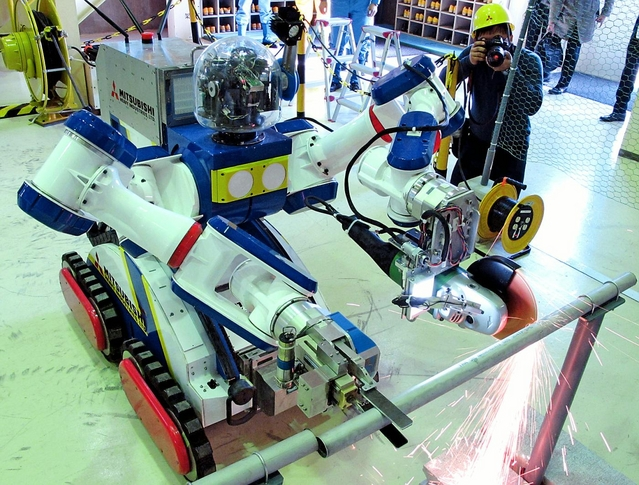
\includegraphics[width=0.98\textwidth]{mhi-meister45.jpg}
			\caption{Coordinated handling of tools by a tele-operated robot \cite{MHI-MEISTeR}}
			\end{figure}
		
		\column{0.6\linewidth}
			
		Human reasoning
		\begin{itemize}
			\item Foresight and adaptiveness to incidents
			\item Superior planning capabilities
		\end{itemize}
		Enhanced flexibility of multiple robots
			\begin{itemize}
				\item Transportation of large/heavy objects
	\item Assembly of multiple parts 
	\item Coordinated use of tools
			\end{itemize}
			
			\end{columns}
\end{frame}

\begin{frame}
	\frametitle{Problem Formulation}

	\begin{itemize}
		\item Precise and stable control during free-motion/contact transition
		\item Enhance versatility by performing friction grasps
		\item (Intuitive) high-level human supervisory control
		\item Local control of formation, independent of the operator
		\item Assistance of the operator with suitable feedback
	\end{itemize}
	
	\begin{block}{Goal}
		Enable a human to \textbf{intuitively} control a robot team executing \textbf{versatile} tasks
	\end{block}	

\end{frame}

\begin{frame}
	\frametitle{Related Work: Robot-team control}
	\begin{itemize}
		\item Virtual object based impedance control \cite{Schneider_92}
				\item Internal and external impedance control \cite{Caccavale_01,Caccavale_08}
			\begin{itemize}
			%\item object tracking required
			%\item knowledge of object shape and dynamics required
			\item Force/Torque sensors at the manipulators required
			\end{itemize}
	
		\item Intrinsically Passive Control \cite{Stramigioli_01, Wimboeck_08}
		\begin{itemize}
			\item no object tracking, virtual object simulation
			%\item knowledge of object shape and dynamics required
		\end{itemize}
		\item Internal impedance control + object dynamics' feed-forward \cite{Erhart_15}
	\item Formation control of a robot team \cite{Sieber_15,Wimboeck_06}
		\begin{itemize}
			\item no object dynamics considered
			%\item no knowledge of object required
		\end{itemize}
	\end{itemize}
\end{frame}

\begin{frame}
	\frametitle{Related Work: Human in the loop}
	\begin{itemize}
		\item Bilateral tele-manipulation  \cite{Lee_05}
		\begin{itemize}
			\item Single master coupled to human, constrained system as slave
			\item Local control of interaction dynamics
			\item Force feedback
		\end{itemize}
		\item Formation-based control \cite{Sieber_15, Scheggi_14}
		\begin{itemize}
			\item Single leader, multiple followers
			\item Robots preserve formation autonomously
			\item Tactile feedback
		\end{itemize}
		\item Gesture-based Control \cite{Gioioso_2014}
		\begin{itemize}
			\item Free-hand motion controls constrained system
			\item Visual feedback
			%\item only visual feedback
		\end{itemize}
		\end{itemize}
\end{frame}

\section{Approach}
\begin{frame}
	\frametitle{port-Hamiltonian system modelling}

	\textbf{Network representation of non-linear physical systems\\}
	\begin{itemize}
	
		\item Mechanical energy storing elements (spring, mass)
		\item Dissipation element (Damper)
		\item Conservative elements (transformer, gyrator)
		\item Interconnection: power port $ \mathcal{P} = \mathcal{V} \times \mathcal{V}^* $ \\ $\mathcal{V}$: space of efforts; $\mathcal{V}*$: (dual) space of flows
		\end{itemize}
		\textit{Example:} Inertia
\[
	\dot{P^b} = C_b \frac{\partial H(P^b)}{\partial P^b} +  W^b \]
	\[T_b^{b,0} = \frac{\partial H(P^b)}{\partial P^b}
\]
$H = \frac{1}{2} (P^b)^T M_b^{-1} P^b$: Hamiltonian energy function;\\ $P^b$: momentum (state); $T_b^{b,0}$: twist (effort); $W^b$: wrench (flow)
		
		
%		\[\begin{pmatrix}\dot{x}_B \\ \dot{x}_S\end{pmatrix} = 
%		\begin{pmatrix}J_B & -Ad_{H_b^0}^T \phi_b^T \\ \phi_b Ad_{H_b^0} & 0\end{pmatrix}
%		\begin{pmatrix}\frac{\partial V}{\partial x_B} \\ \frac{\partial V}{\partial x_S}\end{pmatrix} + \begin{pmatrix}0 & 0 & 0 \\ \phi_v & \phi_i & \phi_{rl}\end{pmatrix}	
%		\begin{pmatrix}T_v^0 \\ T_i^0 \\ T_{rl}^b\end{pmatrix}			 \]
%		\[\begin{pmatrix}W_v^0 \\ W_i^0 \\ W_{rl}^b\end{pmatrix}=
%		\begin{pmatrix}0 & \phi_v^T\\0 & \phi_i^T\\0 & \phi_{rl}^T	
%		\end{pmatrix}
%		\begin{pmatrix}\frac{\partial V}{\partial x_B} \\ \frac{\partial V}{\partial x_S}\end{pmatrix}\]
%		\item Conservative elements (transformer, gyrator)
%			\item Interconnection through power ports
%		\[ \mathcal{P} = \mathcal{V} \times \mathcal{V}^* \]
%		\item Example: variable rest-length spring
%		\begin{eqnarray}\label{EQ:variablerestlengthspring}
%	\dot{H}_i^j =\left( \begin{pmatrix}1 & Ad_{H_b^j}\end{pmatrix} \begin{pmatrix}T_b^{j} \\ T_i^{b}\end{pmatrix} \right) H_i^j\\
%	\begin{pmatrix}W_b^{j,j} \\ W_i^{b,b}\end{pmatrix}  = \left( \begin{pmatrix}1 \\ Ad_{H_b^j}^T\end{pmatrix} \frac{\partial V_{i,j}}{\partial H_i^j} \right) (H_i^j)^T
%\end{eqnarray}

%\end{itemize}

\end{frame}


%\begin{frame}
%	\frametitle{Energy consistent modelling and control}
%	\begin{itemize}
%		\item \emph{Virtual object} concept
%			\begin{itemize}%[leftmargin=0em]
%  				\renewcommand{\labelitemi}{$\Rightarrow$}
%				\item Maps object forces to manipulators
%				\item Stores kinetic energy
%				\item Changes size to adjust formation
%			\end{itemize}
%		\item Model represents energy content of the complete system
%		\item Dampers dissipate energy: \textbf{passive system}
%		\item Operator controls system by energy supply
%			\begin{block}{Stability}
%Model errors never influence passivity nor stability \cite{Stramigioli_01}
%	\end{block}	
%		\end{itemize}
%%\begin{itemize}%[leftmargin=0em]
%%  \renewcommand{\labelitemi}{$\Rightarrow$}
%%\item enhanced human perception through control of a meaningful quantity and appropriate feedback
%%\item stability over a wide class of environments
%%			\end{itemize}
%%		\begin{quote}
%%		If a controlled robot is not passive there is always a passive environment that destabilizes the interconnected system \cite{Stramigioli_15}
%%		\end{quote}
%
%
%\end{frame}


%\begin{frame}
%	\frametitle{Intrinsically Passive Control (IPC)}
%	\begin{columns}
%		\column{0.4\linewidth}
%			
%	
%		\begin{itemize}
%			\item High-level Supervisor and low-level IPC
%			\item IPC + robot: passive
%			\item Power provided by Supervisor
%			\item Environment assumed passive
%		\end{itemize}
%
%		
%		\column{0.58\linewidth}
%             \begin{figure}[htb]
%			\centering
%			%\psfrag{q1}[Bl][Bl]{\small $\alpha$}
%			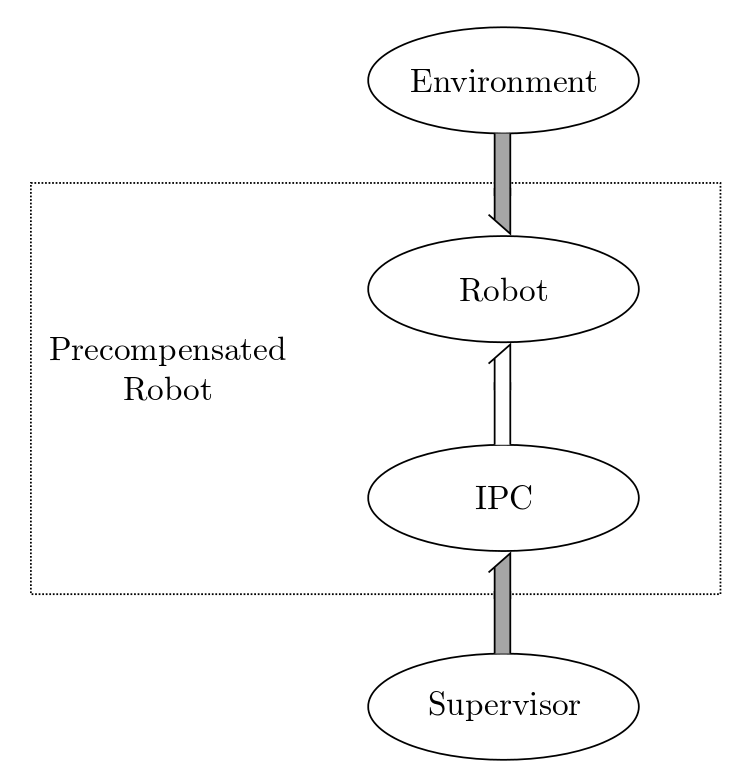
\includegraphics[width=0.9\textwidth]{IPCoverview.png}
%			\caption{Overview of the IPC architecture 								\cite{Stramigioli_01}}
%			\end{figure}
%		
%			
%		\end{columns}
%\end{frame}

\begin{frame}
	\frametitle{Intrinsically Passive Control}
	\textbf{Virtual system model as a controller for the real system}
\begin{columns}[t]
		\column{0.5\linewidth}
			
	
		\begin{itemize}
			\item Geometric interconnection of springs, masses and dampers
			\item Internal and external \emph{impedance} relations
			\item No manipulator inertia re-shaping + dampers: \textbf{passivity}
			\item Energy supplied by operator/environment
			\item Formation changes through variable virtual object shape
		\end{itemize}

		
		\column{0.53\linewidth}
             \begin{figure}[htb]
			\centering
			%\psfrag{q1}[Bl][Bl]{\small $\alpha$}
			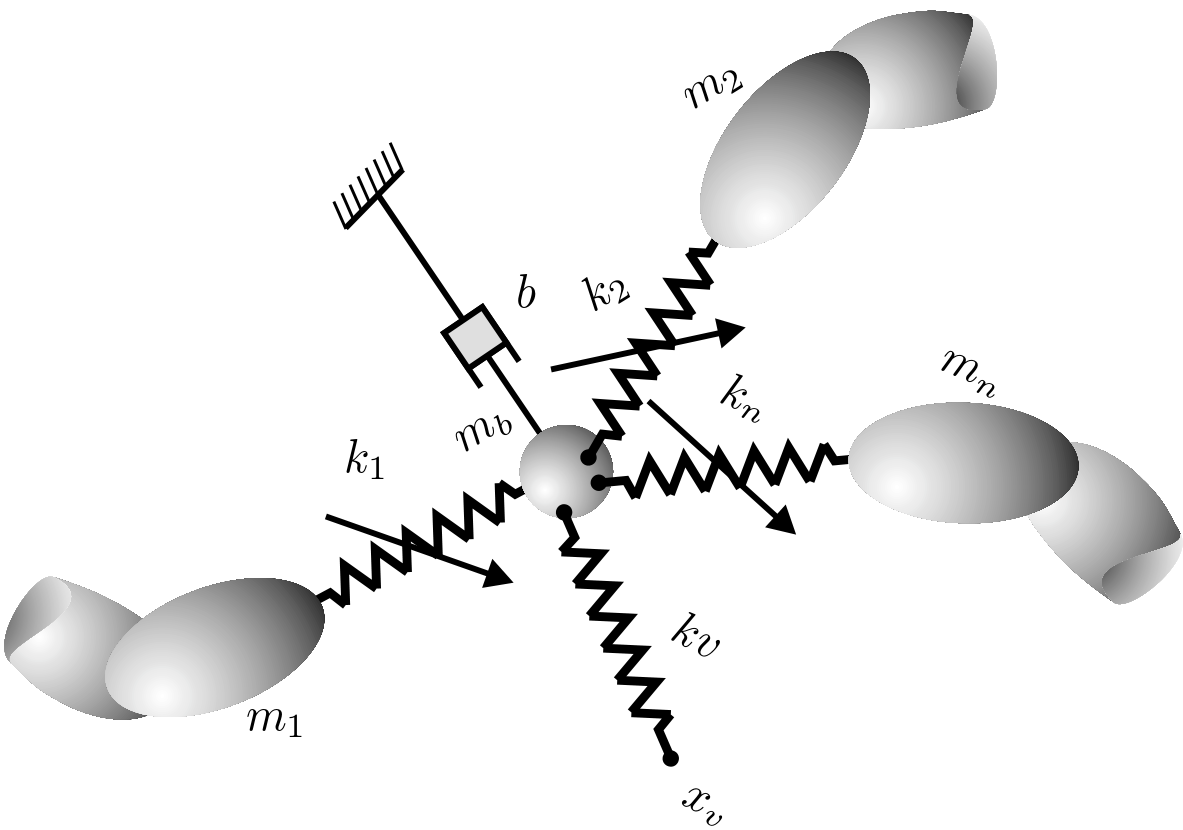
\includegraphics[width=0.9\textwidth]{IPCsprings.png}
			\caption{Mass-spring-damper structure of the IPC \cite{Stramigioli_01}}
			\end{figure}
		
			
		\end{columns}
					\begin{block}{Stability}
Model errors never influence passivity nor stability \cite{Stramigioli_01}
	\end{block}
\end{frame}

\begin{frame}
	\frametitle{Controller Model} \[
	\begin{pmatrix}	\dot{x}_M \\ \dot{x}_S\end{pmatrix} = 
	\begin{pmatrix}J_M & -(\phi_M)^T\\ \phi_M & 0 \end{pmatrix} 
	\begin{pmatrix}\frac{\partial H}{\partial x_M} \\ \frac{\partial H}{\partial x_S}\end{pmatrix}
	+ \begin{pmatrix} 0 & 0 \\ \phi_h & \phi_{rl} \end{pmatrix}
	\begin{pmatrix}
	T_h \\ T_{rl}
	\end{pmatrix}\]
	\[\begin{pmatrix} W_h \\ W_{rl} \end{pmatrix} = 
	\begin{pmatrix}0 & (\phi_h)^T & 0 \\ 0 & (\phi_{rl})^T & 0
\end{pmatrix}\begin{pmatrix}\frac{\partial H}{\partial x_M}\\\frac{\partial H}{\partial x_S}\end{pmatrix} \]
\begin{itemize}


\item $ x_M,x_S $: state vectors of the inertias and springs
\item $H = H_V + H_S + H_M$: sum of energies
\item $J_V,\phi_V,\phi_M,J_M,\phi_h,\phi_{rl}$: geometric description matrices
\item $T_h,T_{rl}$: desired object and rest-length twists
 \item $W_h,W_{rl}$: corresponding wrenches
\end{itemize}
\vspace{10pt}
Reference inputs: $T_h,T_{rl}$\\
Control output: end-effector wrenches $W_E = (\phi_E)^T \frac{\partial H}{\partial x_S} $
	


\end{frame}

%\begin{frame}
%	\frametitle{Grasping an object}
%\begin{columns}
%		\column{0.4\linewidth}
%			
%	
%		\begin{itemize}
%			\item Variable rest-length springs
%			\item Rest-length: virtual object size
%			\item Distinct power port
%		\end{itemize}
%
%		
%		\column{0.62\linewidth}
%             \begin{figure}[htb]
%			\centering
%			%\psfrag{q1}[Bl][Bl]{\small $\alpha$}
%			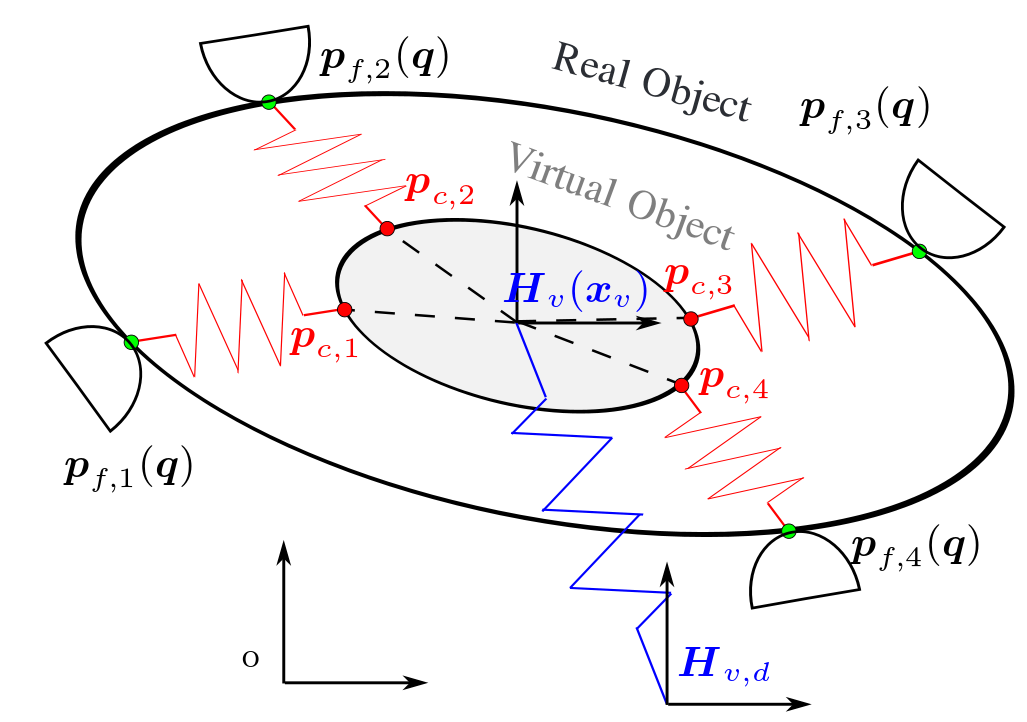
\includegraphics[width=0.98\textwidth]{IPCobjects.png}
%			\caption{Virtual and real object \cite{Wimboeck_08}}
%			\end{figure}
%		
%			
%		\end{columns}
%\end{frame}

\begin{frame}
	\frametitle{Human in the loop}
	\begin{itemize}
			\item Virtual object position is connected with a spring to the desired position
			\item Delays and time-discrete reference changes possibly violate passivity
			\item Passive Set Position Modulation \cite{Lee_10}
			\item Suitable for bilateral tele-manipulation
			\item Spring rest-lengths: adjust to grasp/release objects
		\end{itemize}
		\begin{figure}
					\centering
					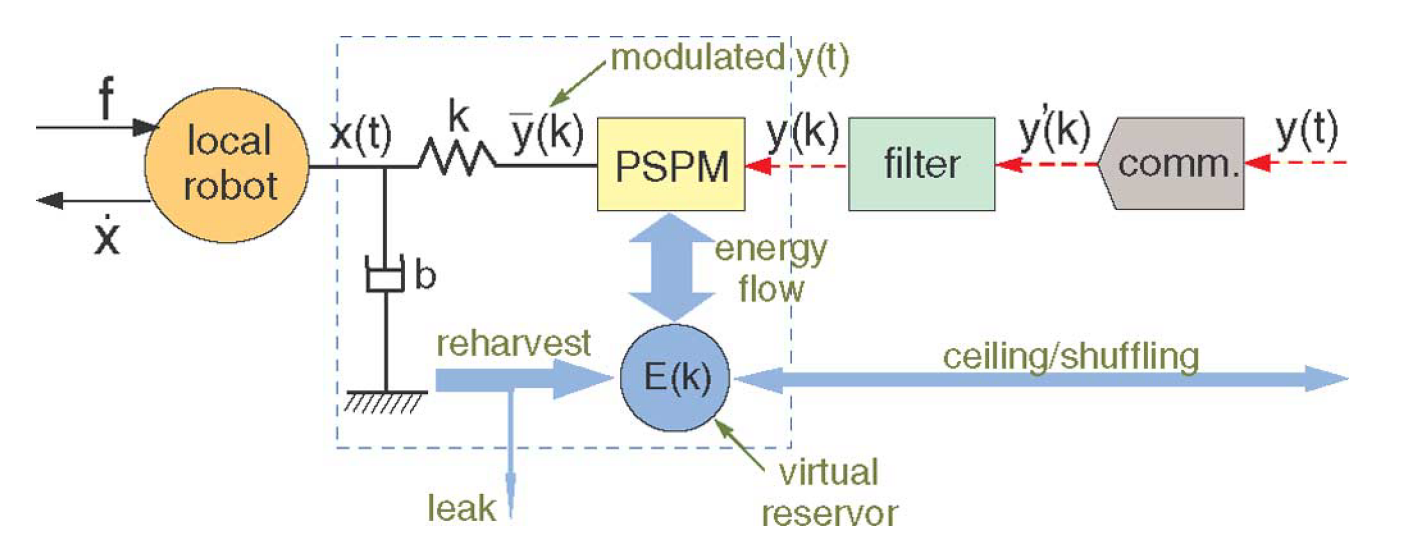
\includegraphics[width=0.8\textwidth]{PSPM.png}
					\caption{Overview over the PSPM\cite{Lee_10}}
		\end{figure}
\end{frame}


\begin{frame}
	\frametitle{Friction grasps: Internal force control}
	Friction constraint of a \emph{soft finger}
	\[f_N \geq \frac{1}{\mu_f} \vert f_T \vert + \frac{1}{\mu_m} \vert m_N \vert
	\]
	\begin{itemize}
		\item Autonomous control of grasping forces subject to dynamic manipulation requirements
		\item Energy taken from virtual object spring
		\item Operator sets constant grasping forces
	\end{itemize}
	
	
\end{frame}

\section{Results}
%\begin{frame}
%	\frametitle{Grasping force optimization for friction contacts}
%	\begin{columns}
%	\column{0.6\textwidth}
%	\begin{itemize}
%	\item required contact normal force is dependent on tangential forces
%	\item high tangential forces arise during acceleration
%	\item other requirements: safety margin, maximum grasping force $\Rightarrow$ cost function
%	\item linear matrix inequality (LMI) problem
%	\end{itemize}
%	\column{0.5\textwidth}
%
%\begin{figure}[htb]
%			\centering
%			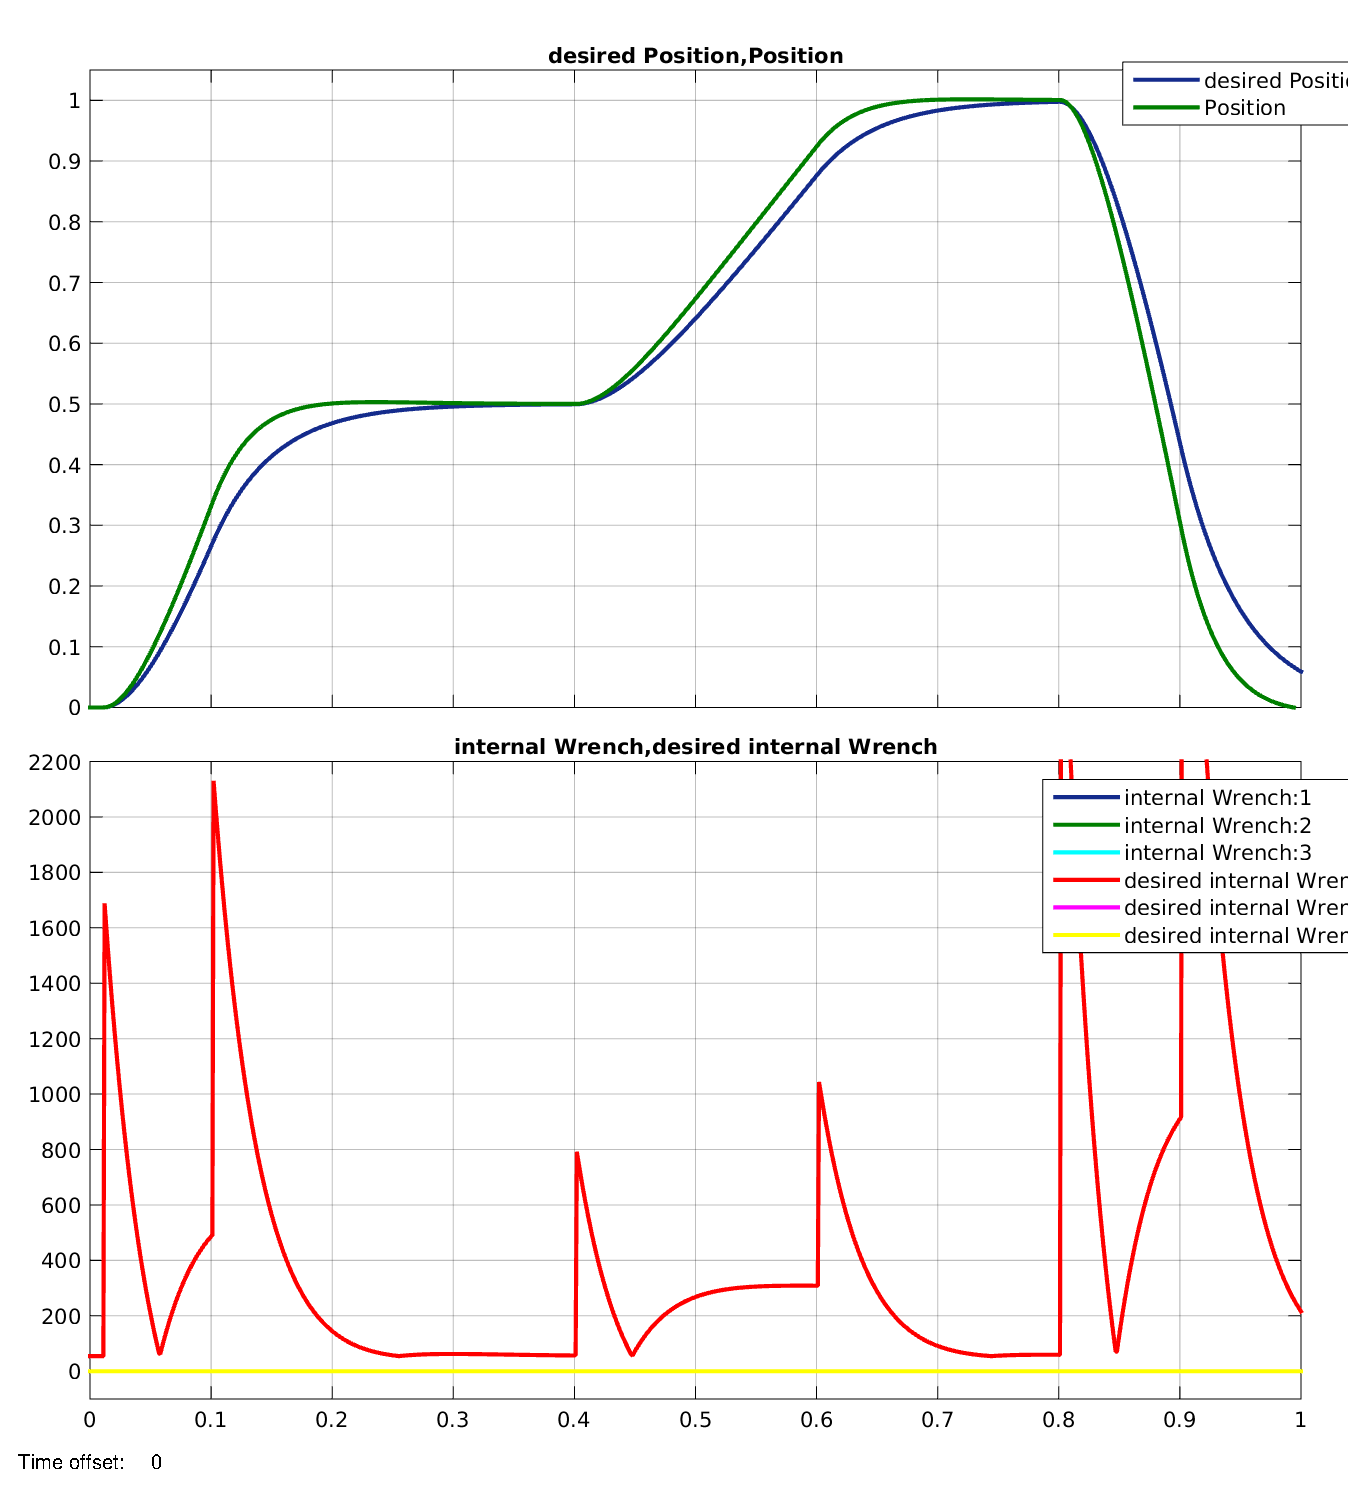
\includegraphics[width=0.9\textwidth]{Hanposforce.eps}
%			\caption{Position, Internal wrench}
%\end{figure}
%\end{columns}
%\end{frame}
\begin{frame}
	\frametitle{Comparison: position tracking}
%Impedance-based reference trajectory generation \cite{Caccavale_01}
\begin{figure}[t]
\begin{tikzpicture}
	\begin{axis} [
		ylabel = {$p_x$[m]},
		xlabel = {t[s]},
		minor y tick num = 1,
		axis lines = left,
		legend entries = {desired position, object force feed-forward, impedance-based trajectory gen., virtual object},
		legend style = {at={(axis cs:1.2, 0.07)}, anchor = north},
		legend cell align=left,
		grid = major,
		height=7.5cm,
		width=0.98\linewidth
	]
\addplot[blue,]
	table {/home/mangerer/MAgit/MA/Latex/plotdata/DePatransdesiredPosition.txt};\addplot[red,]
	table {/home/mangerer/MAgit/MA/Latex/plotdata/DePatransPosition.txt};
\addplot[yellow,]
	table {/home/mangerer/MAgit/MA/Latex/plotdata/CaVi_Position.txt};
\addplot[green,]
	table {/home/mangerer/MAgit/MA/Latex/plotdata/DIPCtransPosition.txt};
\end{axis}
\end{tikzpicture}
%\begin{tikzpicture}
%	\begin{axis} [
%		ylabel = {$p_x$[m]},
%		xlabel = {t[s]},
%		minor y tick num = 1,
%		axis lines = left,
%		legend entries = {position,desired position},
%		legend style = {at={(axis cs:2.6, 0.7)}, anchor = north},
%		legend cell align=left,
%		grid = major,
%		height=3.5cm,
%		width=0.98\linewidth
%	]
%\addplot[red,]
%	table {/home/mangerer/MAgit/MA/Latex/plotdata/DIPCtransPosition.txt};
%\addplot[blue,]
%	table {/home/mangerer/MAgit/MA/Latex/plotdata/DIPCtransdesiredPosition.txt};
%\end{axis}
%\end{tikzpicture}
\vspace{-20pt}
%\caption{Top: Object force feed-forward;
%Bottom: Virtual Object}
\end{figure}
\end{frame}

\begin{frame}
	\frametitle{Comparison: velocity tracking}
%Internal impedance control with object force-feedforward \cite{DePascali_15}
\begin{figure}[t]
\begin{tikzpicture}
	\begin{axis} [
		ylabel = {$v_x$[m/s]},
		xlabel = {t[s]},
		minor y tick num = 1,
		axis lines = left,
		legend entries = {desired velocity, object force feed-forward, impedance-based trajectory gen., virtual object},
		legend style = {at={(axis cs:0.8, -2)}, anchor = north},
		legend cell align=left,
		grid = major,
		height=7.5cm,
		width=0.98\linewidth
	]
\addplot[blue,]
	table {/home/mangerer/MAgit/MA/Latex/plotdata/CaVi_desiredVelocity.txt};
\addplot[red,]
	table {/home/mangerer/MAgit/MA/Latex/plotdata/DePatransVelocity.txt};
\addplot[yellow,]
	table {/home/mangerer/MAgit/MA/Latex/plotdata/CaVi_Velocity.txt};
\addplot[green,]
	table {/home/mangerer/MAgit/MA/Latex/plotdata/DIPCtransVelocity.txt};
\end{axis}
\end{tikzpicture}
%\begin{tikzpicture}
%	\begin{axis} [
%		ylabel = {$v_x$[m]},
%		xlabel = {t[s]},
%		minor y tick num = 1,
%		axis lines = left,
%		legend entries = {velocity,desired velocity},
%		legend style = {at={(axis cs:0.8, -0.5)}, anchor = north},
%		legend cell align=left,
%		grid = major,
%		height=3.5cm,
%		width=0.98\linewidth
%	]
%\addplot[red,]
%	table {/home/mangerer/MAgit/MA/Latex/plotdata/DIPCtransVelocity.txt};
%\addplot[blue,]
%	table {/home/mangerer/MAgit/MA/Latex/plotdata/DIPCtransdesiredVelocity.txt};
%\end{axis}
%\end{tikzpicture}
\vspace{-20pt}
%\caption{Top: External impedance based reference trajectory generation; Bottom: Virtual object}
\end{figure}
\end{frame}

\begin{frame}
	\frametitle{Comparison: internal forces (rotation)}
\begin{figure}[t]

\begin{tikzpicture}
	\begin{axis} [
		ylabel = {f[N],m[Nm]},
		xlabel = {t[s]},
		minor y tick num = 1,
		axis lines = left,
		%legend entries = {force $f_{int,x}$, force $f_{int,y}$, torque $m_{int,z}$},
		%legend style = {at={(axis cs:2.6, 0.04)}, anchor = north},
		%legend cell align=left,
		grid = major,
		height=3.3cm,
		width=0.98\linewidth
	]
\addplot[red,]
	table {/home/mangerer/MAgit/MA/Latex/plotdata/DePaIntWrenchtx.txt};
\addplot[blue,]
	table {/home/mangerer/MAgit/MA/Latex/plotdata/DePaIntWrenchty.txt};
	\addplot[green,]
	table {/home/mangerer/MAgit/MA/Latex/plotdata/DePaIntWrenchrz.txt};\end{axis}
\end{tikzpicture}
\begin{tikzpicture}
	\begin{axis} [
		ylabel = {f[N],m[Nm]},
		xlabel = {t[s]},
		minor y tick num = 1,
		axis lines = left,
		legend entries = {force $f_{int,x}$, force $f_{int,y}$, torque $m_{int,z}$},
		legend style = {at={(axis cs:2.6, 0.1)}, anchor = north},
		legend cell align=left,
		grid = major,
		height=3.3cm,
		width=0.98\linewidth
	]
\addplot[red,]
	table {/home/mangerer/MAgit/MA/Latex/plotdata/DIPCInternalWrenchtx.txt};
\addplot[blue,]
	table {/home/mangerer/MAgit/MA/Latex/plotdata/DIPCInternalWrenchty.txt};
	\addplot[green,]
	table {/home/mangerer/MAgit/MA/Latex/plotdata/DIPCInternalWrenchrz.txt};\end{axis}
\end{tikzpicture}
\vspace{-28pt}
\caption{Top: Object force feed-forward;
Bottom: Virtual Object}
\end{figure}
\end{frame}
\section{Conclusion}

\begin{frame}
	\frametitle{Overview \& open issues}
	\begin{itemize}
		\item Passive control architecture $\Rightarrow$ stability with passive humans and environments
		\item Flexibility through changeable formation
		\item Automatic and passive friction grasp stabilization 
	\end{itemize}
		\begin{block}{Open issues}
\begin{itemize}
\item Formulation of the PSPM in the Hamiltonian framework
\item Energy conservative design of the grasp force assignment
\item Experimental evaluation
\item Evaluation of different human-in-the-loop set-ups
\end{itemize}
	\end{block}	
\end{frame}
\appendix
%\nocite{buss11}
%\nocite{bauer09}
\begin{frame}[allowframebreaks]
	\frametitle{References}
	%\tiny
	%\bibliographystyle{plain}
	%\bibliography{ref}
	\printbibliography
\end{frame}


\end{document}
